\documentclass{report}
\usepackage[utf8]{inputenc}

%----- Configuración del estilo del documento------%
\usepackage{epsfig,graphicx}
\usepackage[left=2.5cm,right=2.5cm,top=1.8cm,bottom=2.3cm]{geometry}
%------ Paquetes matematicos --------%
\usepackage{amsmath}
\usepackage{amssymb}
\usepackage{amsthm}
\usepackage{amsmath}
\usepackage{tabularx}
\usepackage{fancyhdr}
\usepackage{lastpage}
\usepackage{verbatim}
\usepackage[shortlabels]{enumitem}
\usepackage{venndiagram}
\usetikzlibrary{shapes.geometric}
\usepackage{cancel}
\usepackage{hyperref}
\usepackage[T1]{fontenc}
\usepackage[spanish,es-nodecimaldot,es-tabla]{babel}
\usepackage{csquotes}
\usepackage{graphicx}
\usepackage{tocloft}
\graphicspath{{./figs/}}
\usepackage{setspace}
\usepackage{xcolor}


\usepackage[backend=biber]{biblatex}
\addbibresource{resources/referencias/referencias.bib}




\begin{document}
	
	\begin{titlepage}
	\thispagestyle{empty}
	\begin{minipage}[c][0.17\textheight][c]{0.25\textwidth}
		\begin{center}
			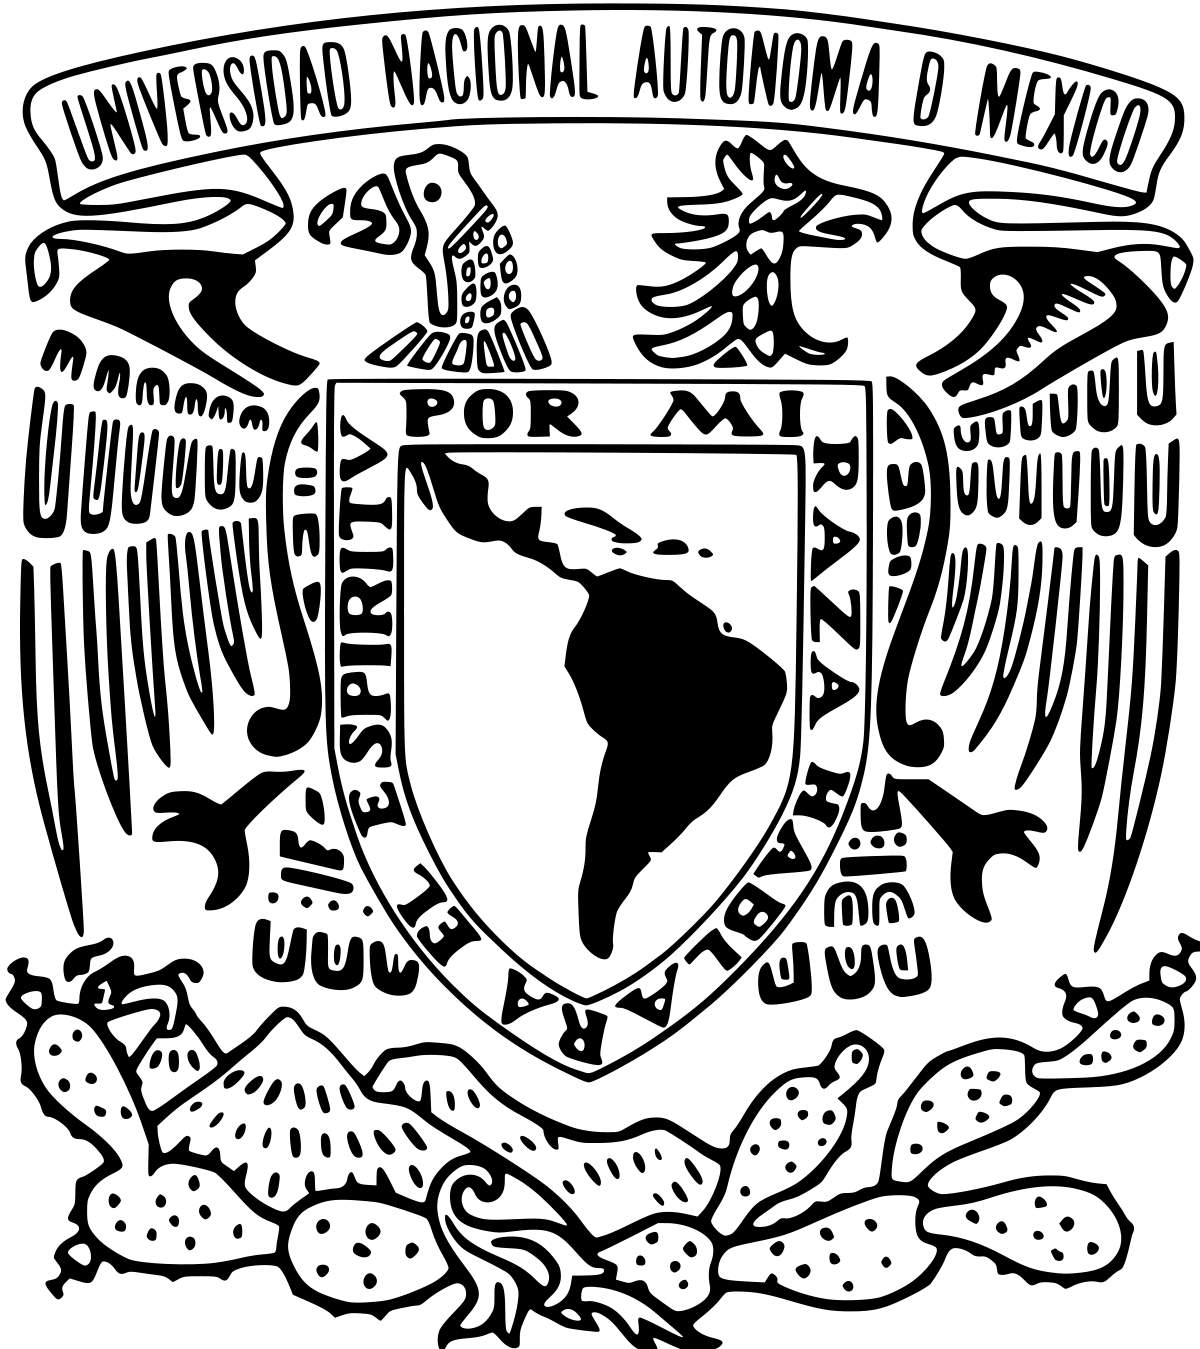
\includegraphics[width=3.5cm, height=3.5cm]{resources/Logo_UNAM.png}
		\end{center}
	\end{minipage}
	\begin{minipage}[c][0.195\textheight][t]{0.75\textwidth}
		\begin{center}
			\vspace{0.3cm}
			\textsc{\large Universidad Nacional Aut\'onoma de M\'exico}\\[0.5cm]
			\vspace{0.3cm}
			\hrule height2.5pt
			\vspace{.2cm}
			\hrule height1pt
			\vspace{.8cm}
			\textsc{Facultad de Ciencias}\\[0.5cm] %
		\end{center}
	\end{minipage}
	
	\begin{minipage}[c][0.81\textheight][t]{0.25\textwidth}
		\vspace*{5mm}
		\begin{center}
			\hskip2.0mm
			\vrule width1pt height13cm 
			\vspace{5mm}
			\hskip2pt
			\vrule width2.5pt height13cm
			\hskip2mm
			\vrule width1pt height13cm \\
			\vspace{5mm}
			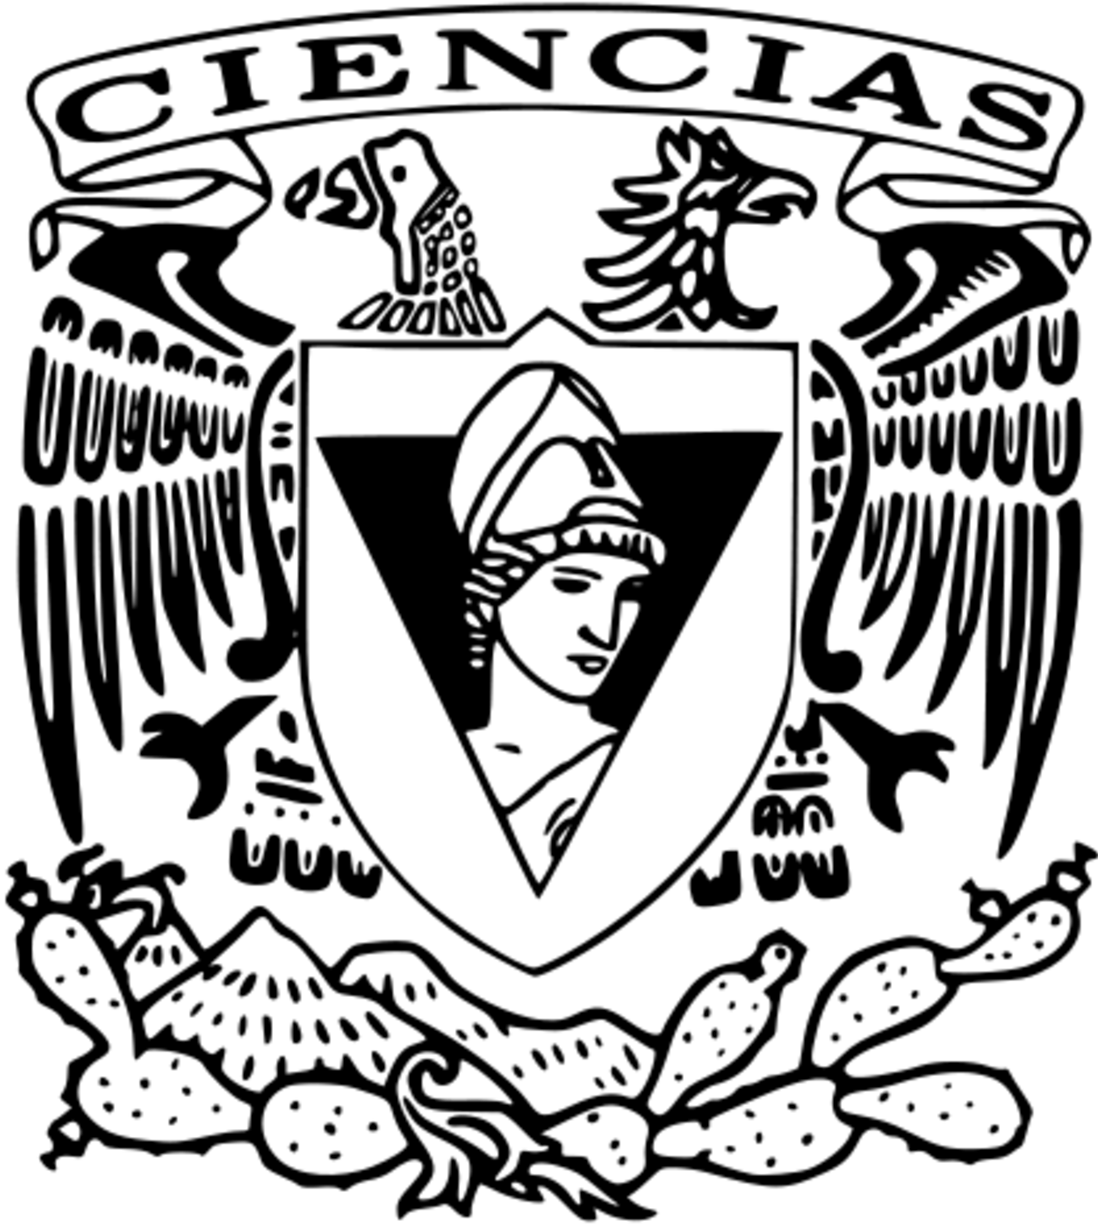
\includegraphics[height=4.0cm]{resources/Logo_FC.png}
		\end{center}
	\end{minipage}
	\begin{minipage}[c][0.81\textheight][t]{0.75\textwidth}
		\begin{center}
			\vspace{1cm}
			
			{\large\scshape Fundamentos de Bases de Datos - 7094}\\[.2in]
			
			\vspace{2cm}            
			
			\textsc{\LARGE \textbf{T}\hspace{1cm}\textbf{A}\hspace{1cm}\textbf{R}\hspace{1cm}\textbf{E}\hspace{1cm}\textbf{A}\hspace{1cm}\hspace{1cm}\textbf{4}}\\[2cm]
			\textsc{\Large{Equipo:}\normalsize \\
                \vspace{.3cm}
				\textbf{Del Monte Ortega Maryam Michelle - 320083527 \\
                \vspace{.2cm}
				\href{https://github.com/JuanSosaCiencias}{\textcolor{blue}{Sosa Romo Juan Mario - 320051926}} \\
                \vspace{.2cm}
				Castillo Hernández Antonio - 320017438 \\
                \vspace{.2cm}
                Erik Eduardo Gómez López - 320258211 \\
                \vspace{.2cm}
                Julio César Islas Espino - 320340594}}\\[0.5cm]     
			
			\textsc{{Fecha de entrega: \\ \textbf{10 de Octubre de 2024}}}\\[0.5cm]        
			
			\textsc{{Profesor: \\ \textbf{M. en I. Gerardo Avilés Rosas}}}\\[0.5cm]  
			
			\textsc{Ayudantes: \\ \textbf{Luis Enrique García Gómez \\ Kevin Jair Torres Valencia \\ Ricardo Badillo Macías \\ Rocío Aylin Huerta González
			} }
			
			
			\vspace{0.5cm}
		\end{center}
	\end{minipage}
\end{titlepage}

	
	\begin{center}
		\section*{\LARGE{Practica 3}}
	\end{center}
    \begin{center}
        \LARGE{\textbf{Modelo Entidad Relación Extendido:}}\\
    \end{center}
    \normalsize
    \input{ERE/ere.tex}

    % Preguntas  
    \begin{center}
        \LARGE{\textbf{Restricciones importantes:}}\\
    \end{center}
    \normalsize

    

Restricciones importantes que incorporamos:

Para atleta, entrenador y arbitro hemos decidido que sean entidades hijas de Persona, ya que todas comparten que deben tener los mismo datos básicos

Realizamos agregación en la parte de medallero ya que necesitamos involucrar qué \textbf{atletas} ganaron medallas, es decir, cuáles son \textbf{ganadores} y de ahí contabilizar las medallas en los \textbf{países}. 

En la relación Ser Ganador hemos decidido guardar el Número de medallas para los países, esto para contabilizar al final cuántos atletas de medalla de oro (plata, o bronce según el caso) tiene determinado país y asignar el Medallero.

Localidad que dependerá de que haya una disciplina en el lugar, por ello, Localidad también guardará el nombre de la Disciplina que impartirá.

\begin{center}
    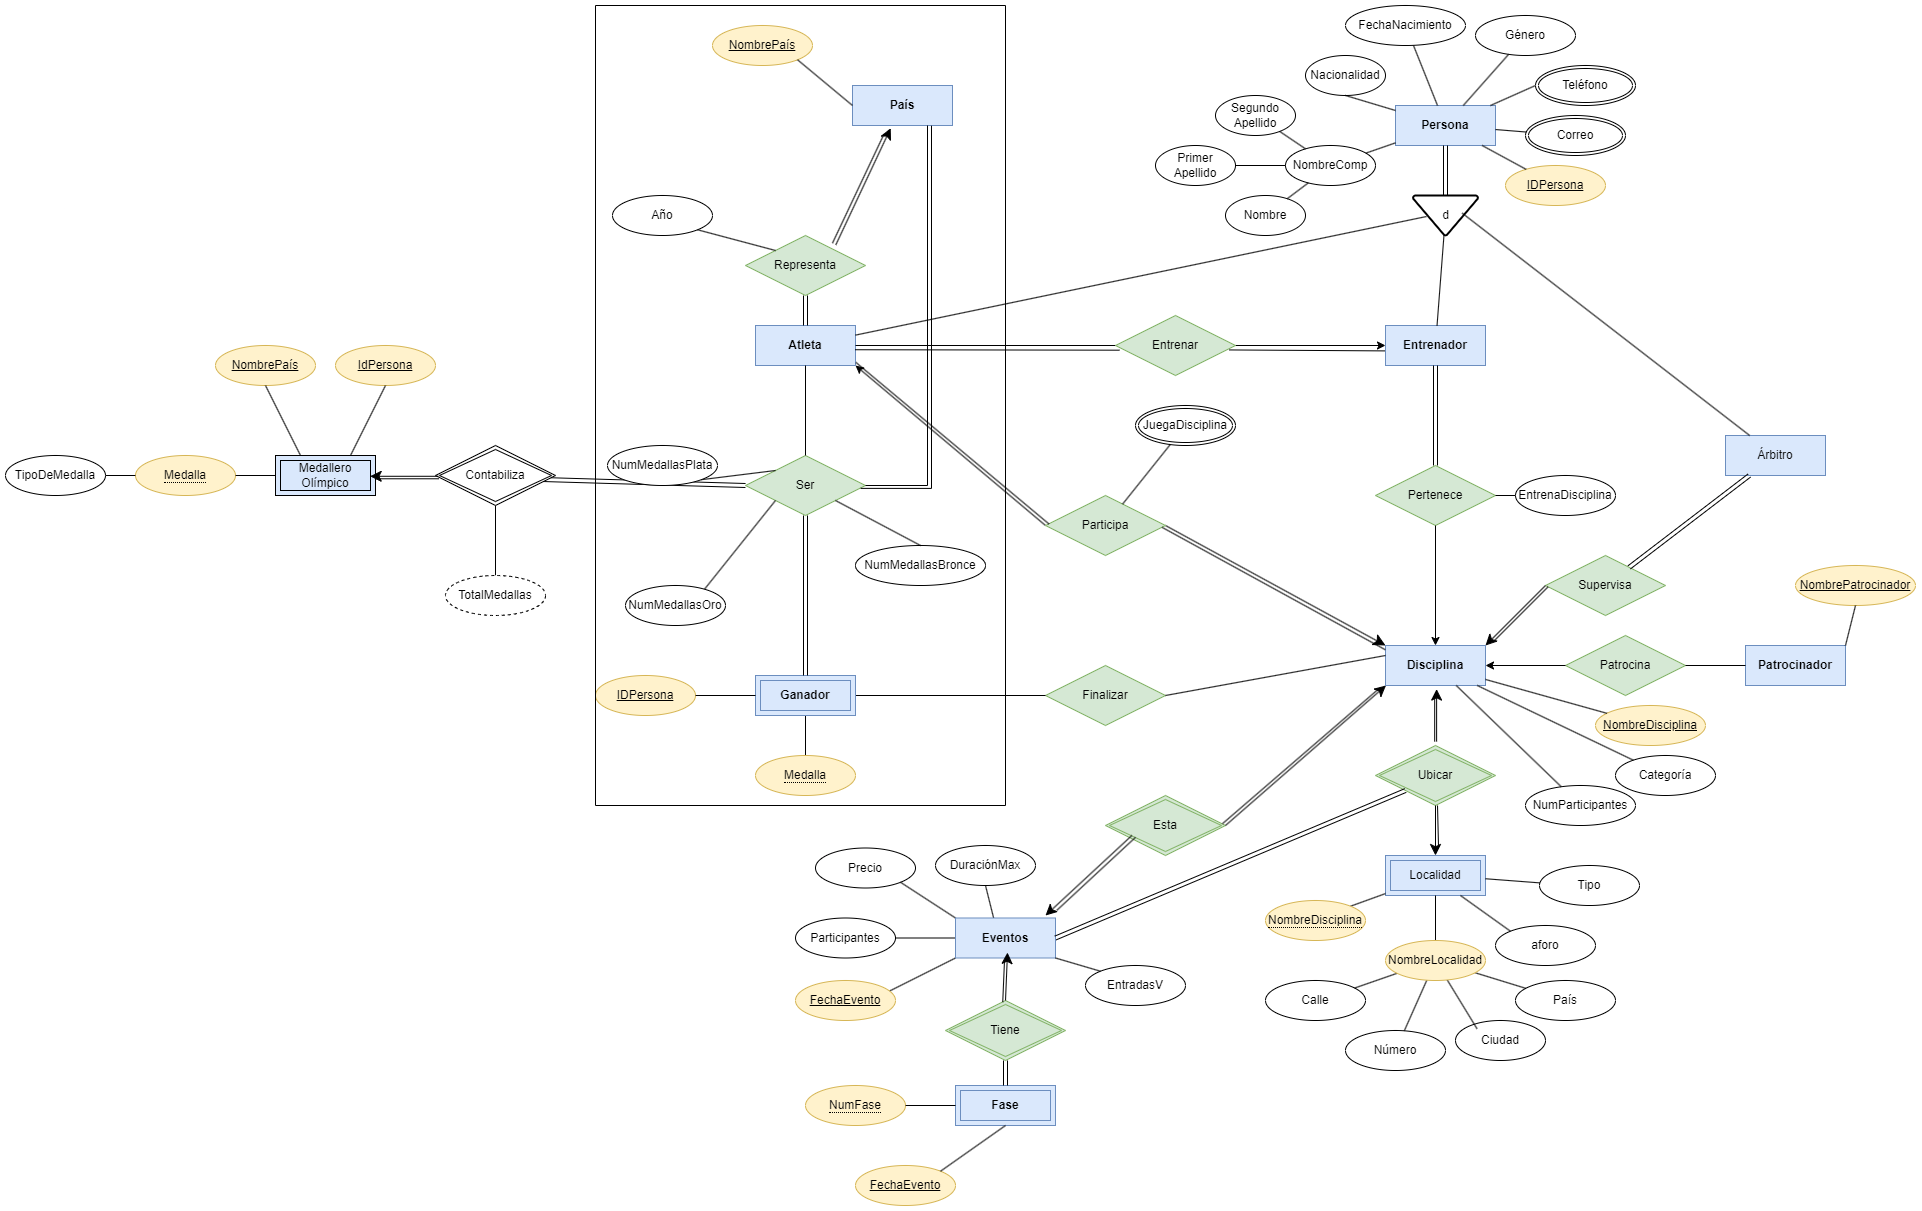
\includegraphics[width=17cm]{resources/DiagramaOlimpiadas.png}
\end{center}



    \newpage
    
\printbibliography
  
\end{document}